%%%%%%%%%%%%%%%%%%%%%%%%%%%%%%%%%%%%%%%%%%%%%%%%%%%%%%%%%%%%%%%%%%%%%%%%%%%%%
%%% A Dependency Network+Weigthed Kernel Approach for Feature Selection
%%% Proposal for a MSc Project
%%% Nestor Rodriguez + Sergio A. Rojas (c) 2010
%%%
%%% Main file for the MSc proposal 
%%%%%%%%%%%%%%%%%%%%%%%%%%%%%%%%%%%%%%%%%%%%%%%%%%%%%%%%%%%%%%%%%%%%%%%%%%%%%

%------------------------------ Document header -----------------------------

% Set document type: MSc report
\documentclass[a4paper,twoside,12pt]{article}

% Include needed packages
\usepackage{graphicx}             	    % For including graphics in EPS
\usepackage{amsmath,amssymb,amsthm}      % For American Maths Society math
\usepackage{setspace}                    % For line spacing
\usepackage{cite}                        % For doing citations
\usepackage[vcentering,dvips]{geometry}  % For layout and margins settings
\usepackage{algorithm,algorithmic}		% For algorithms	
\usepackage{pdfcomment}
\usepackage{pdflscape}
\usepackage{hyperref}
\usepackage[svgnames,rgb]{xcolor}%

% Set layout and margins
\geometry{a4paper,left=1.0in,right=1.0in,top=1.0in,bottom=1.0in}
\bibliographystyle{plain}

% Set figures path
\graphicspath{{figs/}}

% Notation
\newcommand{\cD}{{\cal D}}
\newcommand{\cA}{{\cal A}}
\newcommand{\bomega}{{\boldsymbol{\omega}}}
\newcommand{\cN}{{\cal N}}
\floatname{algorithm}{Algorithm}
\renewcommand{\algorithmicrequire}{\textbf{Inputs:}}
\renewcommand{\algorithmicensure}{\textbf{Outputs:}}
\renewcommand{\algorithmicrepeat}{\textbf{repeat}}
\renewcommand{\algorithmicuntil}{\textbf{until}}
\renewcommand{\algorithmicfor}{\textbf{for}}
\renewcommand{\algorithmicdo}{\textbf{do}}
\renewcommand{\algorithmicend}{\textbf{end}}
\renewcommand{\thefootnote}{\fnsymbol{footnote}}
\pdfcommentsetup{icon=Comment,color=Khaki, open=true}
\defineavatar{reviewer}{author=Marco A. Alzate}
\defineavatar{me}{author=Nestor Andres Rodriguez}

\hypersetup{
    colorlinks,%
    citecolor=black,%
    filecolor=black,%
    linkcolor=black,%
    urlcolor=black
}


%------------------------------ Document body -------------------------------
\begin{document}
%%%%%%%%%%%%%%%%%%%%%%%%%%%%%%%%%%%%%%%%%%%%%%%%%%%%%%%%%%%%%%%%%%%%%%%%%%%%%
%%% A Dependency Network+Weigthed Kernel Approach for Feature Selection
%%% Proposal for a MSc Project
%%% Nestor Rodriguez + Sergio A. Rojas (c) 2010
%%%
%%% This is the title page for the proposal
%%%%%%%%%%%%%%%%%%%%%%%%%%%%%%%%%%%%%%%%%%%%%%%%%%%%%%%%%%%%%%%%%%%%%%%%%%%%%

\singlespacing
\title{Feature relevance estimation by evolving probabilistic dependency networks with weighted kernel machines
\footnote{\tiny A MSc thesis proposal}}
\date{\today}
\author{Nestor Rodriguez \pdfcomment[avatar={me}]{The comments inside the whole document contain your observations together with their respective corrections and clarifications.} \footnote{\tiny Engineering School, District University of Bogota, Colombia}  \\ \small{\textbf{Advisor:} Sergio A. Rojas, PhD.}}

\maketitle

\begin{abstract}
\addtocounter{footnote}{2}
This thesis proposal focuses on the problem of estimating relevance of observed variables for a classification task in high dimensional spaces, which is known as feature subset selection or feature relevance determination by the machine learning community. The main goal of the thesis is the design of a novel feature relevance estimation method by combining techniques for estimation of probabilistic dependency networks with weighted kernel machines\footnote{\tiny The topics of feature selection methods, estimation of probability distribution algorithms and kernel machines are briefly reviewed in section \ref{sec:lecrev}. The interested reader is referred to \cite{guyon03,heckerman99, cristianini04} for details.}. The method is intended to work within a population-based stochastic search framework where relevant (but unknown) variables from a given dataset\footnote{\tiny In the context of this paper \emph{dataset} means data arranged in a tabular way where columns represent variables and rows represents instances.  Other types of formats (such as text, images, graphs, etc.) are not considered.} are found by iteratively evolving a set of relevance estimation candidates. These candidates will consist of parameters of multivariate conditional probability distributions. The distributions could be seen as dependency networks of how variables influence each other.  With this information a subset of the most relevant features from the original sample can be selected to perform classification, the suitability of the subset being assessed as its predictive classification accuracy. Weighted kernel classifiers would be used for this purpose. It is expected that the method may provide additional information about dependency among such variables as a byproduct of the selection process.
\end{abstract}



\clearpage
\tableofcontents 
\listofalgorithms \listoffigures %\listoftables 
\clearpage
\setlength{\parskip}{5mm plus1mm minus2mm} 
%%%%%%%%%%%%%%%%%%%%%%%%%%%%%%%%%%%%%%%%%%%%%%%%%%%%%%%%%%%%%%%%%%%%%%%%%%%%%
%%% A Dependency Network+Weigthed Kernel Approach for Feature Selection
%%% Proposal for a MSc Project
%%% Nestor Rodriguez + Sergio A. Rojas (c) 2010
%%%
%%% Chapter 2: Formulation
%%%%%%%%%%%%%%%%%%%%%%%%%%%%%%%%%%%%%%%%%%%%%%%%%%%%%%%%%%%%%%%%%%%%%%%%%%%%%
\section{Problem, Motivation and Research Hypothesis}
\subsection{Problem and Motivation}
\label{sec:formulation}

Feature subset selection (FSS) is a machine learning technique for dimensionality reduction in datasets where irrelevant or noisy variables may appear. It is useful in problems where few from a big set of observed variables explain a given pattern in classification, prediction or clustering of data cases (e.g. diagnosis of a disease, market analysis, image segmentation, etc.), and therefore it allows for an expert to focus on data that is really important, reducing the expenditure of costly or time-consuming experiments.  

To illustrate the problem, consider the situation where an insurance company is evaluating the factors that have an impact on people's overweight conditions that lead to claims in illness insurance policies. Upon registration, they collect information of both parents' weight and birthday. They want to know which of these variables are related to the development of the condition. Now let us suppose that one-year time is required by an insurance analyst to process the information of just one variable. Then it would be desirable to discard irrelevant variables in order to save him valuable time. An FSS method could help to select the relevant ones.

\begin{figure}[h]
	\centering
		\includegraphics{Images/example01}
	\caption[Correlation analysis of input variables in relation to overweight conditions of insurance customers.]%
	{Correlation analysis of input variables in relation to overweight conditions of insurance customers (for the fictional example in the text).}
	\label{fig:im01}
\end{figure}

Figure \ref{fig:im01} depicts the result of applying a correlation-based feature selection method on this fictional problem; it is evident that half of the variables, namely those related to birth dates, are irrelevant and can be ignored for the problem of interest. Thus, dimensionality reduction may provide insights in data mining tasks, yielding a better understanding of objects or phenomena behavior and is useful to speed up data analysis and to improve generalization performance. For instance, in the previous insurance company example, Figure \ref{fig:im08} shows how sample cases can be now rendered in the 2D space obtained with the relevant variables; they can be easily discriminated with a simple hyperplane. By focusing on those two relevant variables, the analyst would have saved two precious years of working time and the company two equally valuable years of salary payments. 

\begin{figure}[h]
	\centering
		\includegraphics{Images/example02.png}
	\caption{Using relevant features customers can be easily segmented with a simple linear function.}
	\label{fig:im08}
\end{figure}

Some FSS techniques assume variables are independent.  This assumption might not be appropriate for some real world problem since variables may influence others and these interactions are usually hidden.  A good example is in the field of bioinformatics where experts analyze proteins relevance in diseases to design inhibitory vaccines; using state-of-the-art high-throughput technologies (e.g. mass-spectometry\cite{lipton08}) they are able to collect large amounts of data about activation of protein mechanisms, but the information about how these interactions occur is unknown or difficult to obtain, not to mention that just a few proteins from a large proteomic spectrum would be related to the activation of the disease. 

The independent assumptions (univariate FSS methods, see section \ref{sec:feat1}) are very popular because of their low computational cost\cite{larranaga08} but they do not provide additional insights about data relationships.  On the other hand, missing information about those dependencies may affect negatively the prediction accuracy of the feature subset.  As an alternative approach, multivariate FSS methods search for feature subsets and possible dependency relationships between them at the cost of an increase in computational complexity (recall that FSS is a combinatorial problem known to be NP-Hard \cite{guyon03,rojas05}). The challenge is then to design novel feature selection methods that take advantage of multivariate power combined with high-accuracy classifiers to obtain improved prediction and explanatory performance.

On the other hand, kernel classifiers have recently emerged as powerful high-accuracy classifiers with robust generalization abilities \cite{cristianini04}.  They use linear functions to perform classification, allowing for non-linear discriminatory borderlines in the input space by means of a kernel function. This function is a mapping of similarity measures in a transformed space where nonlinearities can be solved linearly. Two widely used kernel functions are the RBF kernel and the polynomial kernel (Eq.(\ref{eq:eq01}) and Eq.(\ref{eq:eq02}) respectively):

\pdfcomment[avatar={reviewer}, id=5]{5.1 Whenever a mathematical symbol is used, it should be clearly defined. }
\pdfreply[avatar=me, id=50, replyto=5]{Symbols in equations and algorithms were clearly defined.}
\begin{equation}
	K_{\sigma}(\bar{x},\bar{z}) = \text{exp}\Big( -\sigma\sum_{k} (x_k-z_k)^2 \Big)
	\label{eq:eq01}
\end{equation} and
\begin{equation}
	K_d(\bar{x},\bar{z}) = \langle \bar{x}, \bar{z} \rangle^d,
	\label{eq:eq02}
\end{equation} where \(\bar{x}, \bar{z} \in X\), \(X \subseteq \mathbb{R}^D \) represents the input space and {\scriptsize $D$ } the number of variables or dimensions.  The parameter \(\sigma\) and \(d\) define the width of the RBF and polynomial kernel respectively.  Modified weighted versions of these kernels introduce scale factors \(\bar{w} = \{w_1...w_\ell\}\) to weight the amount that each dimension contributes to the total computation\cite{vapnik02}.  The weighted RBF and weighted polynomial kernels are then defined as Eq.(\ref{eq:eq03}) and (\ref{eq:eq04}):

\begin{equation}
	K_{\sigma}(\bar{x},\bar{z}) = \text{exp}\Big( -\sigma \sum_{k}^{\ell} w_k(x_k-z_k)^2 \Big)
	\label{eq:eq03}
\end{equation} and

\begin{equation}
	K_{d}(\bar{x},\bar{z}) = \Big( \sum_{k}^{\ell} w_k(x_k \cdot z_k) \Big)^d.
	\label{eq:eq04}
\end{equation}

Some FSS methods have been proposed in connection with kernel functions, for instance the weighted kernels in Eq. (\ref{eq:eq03}) and (\ref{eq:eq04}) have been used to define a FSS embedded method (the weigthed kernel iterative estimation of relevance algorithm, wKIERA\cite{rojas08}).  The idea in this case is to consider the weight vector \(\bar{w}\) of the kernel as a relevancy estimator of input variables. The vector is tuned by a univariate estimation of distribution algorithm \cite{larranaga01} which iteratively refines the distribution by a population-based technique inspired in genetic algorithms (GA)\cite{goldberg89}. The accuracy of the kernel classifier coupled with the weight vector candidates is taken as the fitness measure of the GA.  The authors showed promising results of this algorithm in selecting relevant variables in a number of different classification tasks, including problems with linear and non-linear hypothesis targets. This FSS method however, is designed on the basis of the independent assumption mentioned above and consequently does not provide the power of explanation of multivariate methods and does not account for information of relationship between the variables. One of the motivations of this thesis proposal is to build upon this method and design a refined version that incorporates techniques for multivariate feature selection within an embedded population-based stochastic algorithm. Dependency networks, also known as belief or Bayes networks \cite{heckerman99}, would be preliminary chosen to represent how variables depend and influence each other, and one of the goals of the thesis is to design and new algorithms to perform relevance estimation within such framework and to make feasible the approach. 

Finally, it is worth to note that the work by \cite{larranaga00FSS} propose a FSS multivariate method that accounts for dependencies between variables by estimating belief networks. Their approach however is a wrapper method (see section \ref{sec:feat1}) and they do not incorporate the powerfulness of nonlinear kernel classifiers. We will however review this study, and as far as possible compare the different approaches.

\subsection{Research Hypothesis} 
\pdfcomment[avatar={reviewer}, id=1]{It is convenient to establish the problem as a research hypothesis to be tested, in order to clarify
 the contributions and facilitate the evaluation of the research project.}
 \pdfreply[id=10,avatar={me},replyto=1]{This section presents the missing research hypothesis.}

We will consider the following research hypothesis: Given a set of observations taken from a particular phenomenon where dependencies among variables exist but are hidden, it is feasible to select a subset of variables that are relevant in a classification task with a method that combines iterative estimation of dependency networks coupled with weighted-kernel classifiers, in order to produce a predictor model that improves the understanding of the problem domain when compared with other techniques based on independence assumptions.
\clearpage
%%%%%%%%%%%%%%%%%%%%%%%%%%%%%%%%%%%%%%%%%%%%%%%%%%%%%%%%%%%%%%%%%%%%%%%%%%%%%
%%% A Dependency Network+Weigthed Kernel Approach for Feature Selection
%%% Proposal for a MSc Project
%%% Nestor Rodriguez + Sergio A. Rojas (c) 2010
%%%
%%% Chapter 3: Acknowledgements
%%%%%%%%%%%%%%%%%%%%%%%%%%%%%%%%%%%%%%%%%%%%%%%%%%%%%%%%%%%%%%%%%%%%%%%%%%%%%

\section{Idea and Proposal}
\label{sec:IdAndProp}

The new FSS method will involve the following main components (see Figure \ref{fig:im02}). The \emph{data}, which is the sample of observed variables for a given problem; the overall goal of the method will be to identify relevant feature subsets and as much as possible information about dependencies that explain significant patterns hidden in the data.  The \emph{dependency network model} represents the relationships among variables and how they affect each others.  

\begin{figure}[ht]
	\centering
		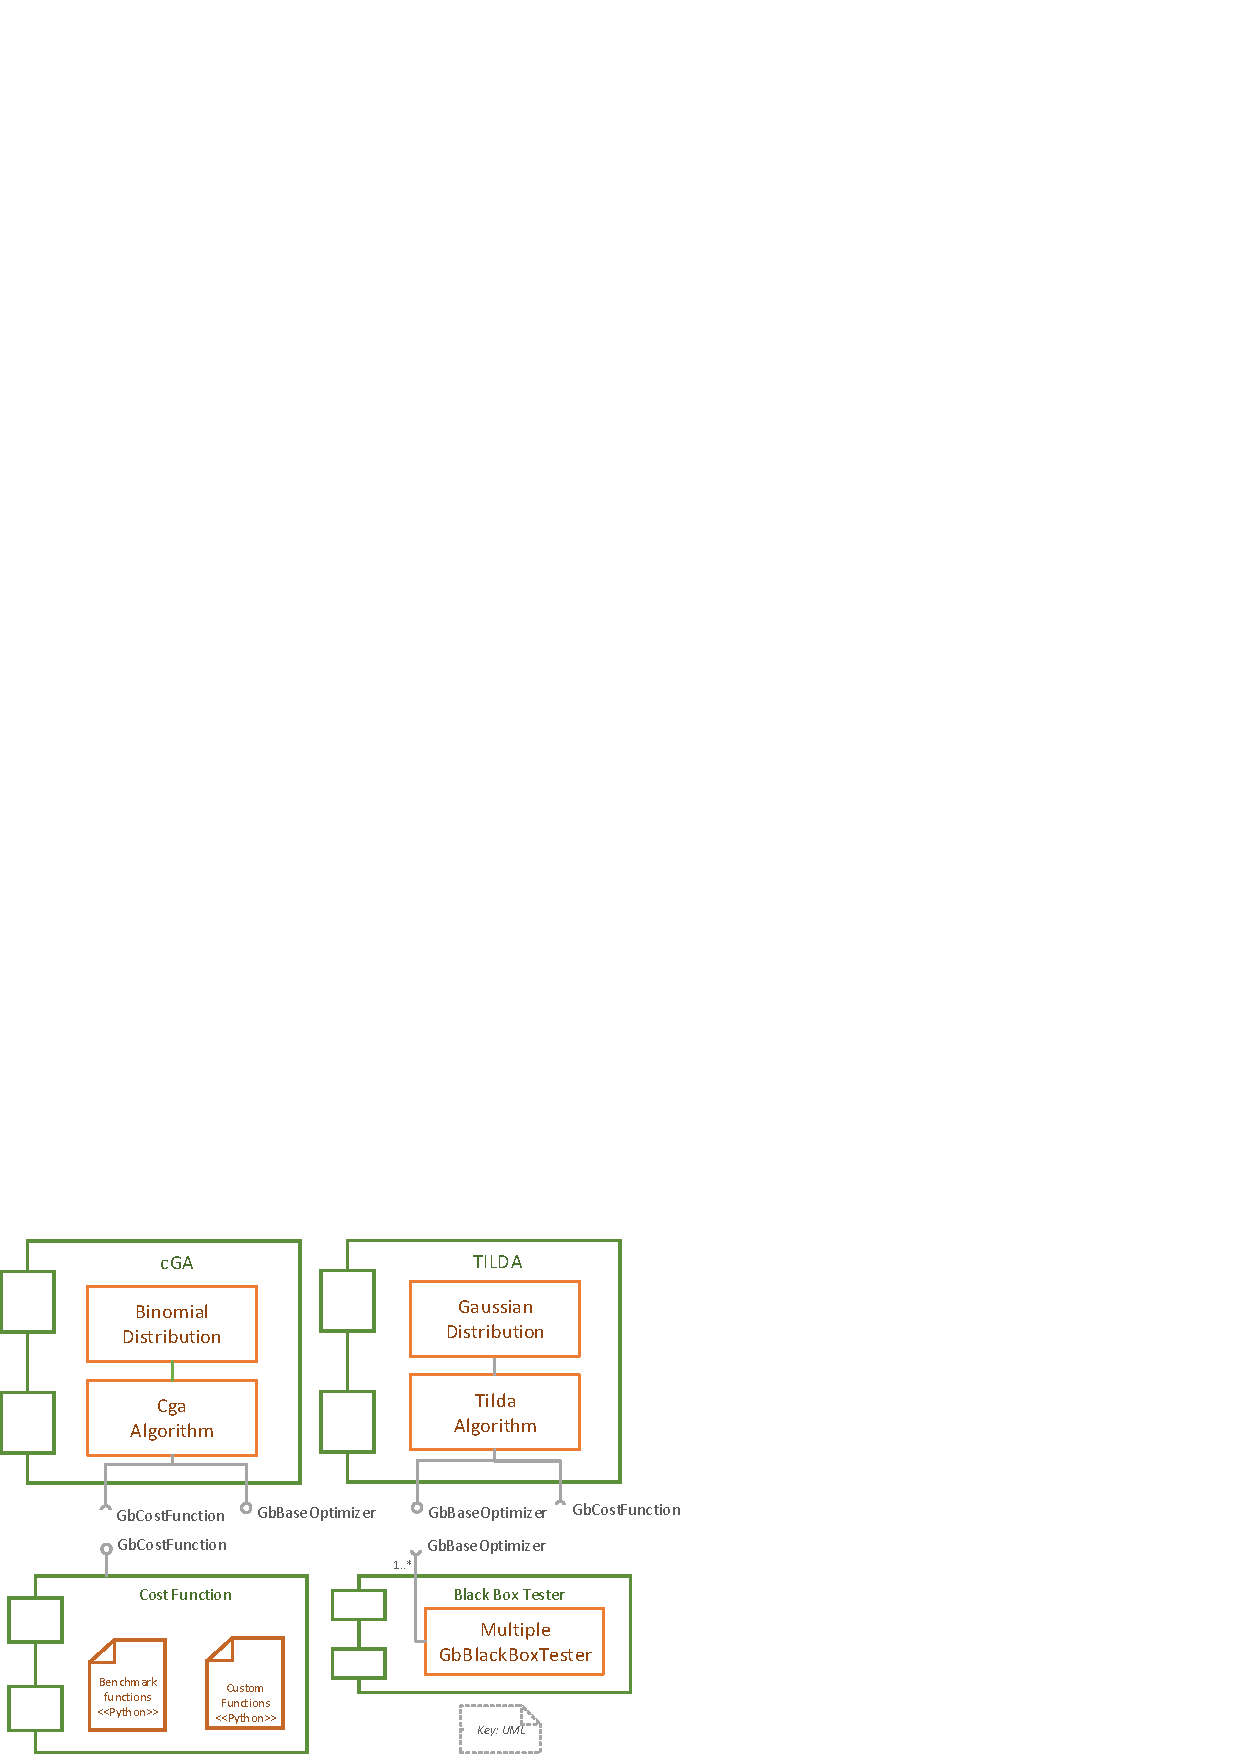
\includegraphics{Images/components.jpg}
	\caption{The components involved in this thesis proposal.}
	\label{fig:im02}
\end{figure}

The \emph{multivariate estimation of distribution algorithm} is a technique to infer the parameters and structure of the dependency network by estimating a probability distribution of relevancy from a pool of candidate weight vectors; the distribution and candidates are adjusted within a framework of a stochastic population-based evolutionary algorithm. Lastly, the \emph{weighted kernel classifier} will perform the iterative classification using relevant feature subsets according to the evolved relevance distributions.

A draft schematic flowchart of the conceived method is shown in Figure \ref{fig:im03}. Preliminary pseudo-code of the method is summarized in Algorithm \ref{alg:idea}.

\begin{figure}[ht]
	\centering
		\includegraphics{Images/flowchart.png}
	\caption{Preliminary depiction of the expected method described in this proposal.}
	\label{fig:im03}
\end{figure}

\begin{algorithm}[ht]
	\caption{\textsf{Preliminary pseudocode of the expected method described in this proposal}}
	\begin{algorithmic}
		\REQUIRE Given a dataset $\cD$, a weighted kernel $\kappa_\omega$ and a classifier $\cA$
		\STATE Let $\beta$ represents a dependency network distribution initialized with an independent joint distribution.
		\REPEAT 
			\STATE Split $\cD$ in training $\cD_{t}$ and testing $\cD_{s}$ data
			\STATE $\bar{\Omega} \gets$ Sample $k$ candidates from $\beta$ \pdfcomment[avatar={reviewer}, id = 7]{In algorithm 1 the first set of k candidates is taken from an empty set} \pdfreply[avatar=me, id= 70, replyto=7]{ \emph{Beta} represents a dependency network distribution. Thus in the first algorithm iteration the k candidates are not sample from an empty set but rather from an independent joint distribution. }
			\FOR{$\bomega_j \in \Omega$}
				\STATE Train classifier: $h_j \gets \cA (\cD_{t}, \kappa_{\omega_j})$
				\STATE Test classifier: $e_j \gets$ error$(h_j, \cD_{s}, \kappa_{\omega_j})$
			\ENDFOR
			\STATE $\bar{\Omega}' \gets$ bestCandidates$(\bar{\Omega},\bar{e})$
			\STATE Re-estimate dependency network: $\beta \gets$ reEstimate$(\bar{\Omega}')$
	\UNTIL $\beta$ has converged or maximum number of iterations reached
	\end{algorithmic}
	\label{alg:idea}
\end{algorithm}
\clearpage
%%%%%%%%%%%%%%%%%%%%%%%%%%%%%%%%%%%%%%%%%%%%%%%%%%%%%%%%%%%%%%%%%%%%%%%%%%%%%
%%% A Dependency Network+Weigthed Kernel Approach for Feature Selection
%%% Proposal for a MSc Project
%%% Nestor Rodriguez + Sergio A. Rojas (c) 2010
%%%
%%% Chapter 1: Introduction
%%%%%%%%%%%%%%%%%%%%%%%%%%%%%%%%%%%%%%%%%%%%%%%%%%%%%%%%%%%%%%%%%%%%%%%%%%%%%

\section{Goals}
\label{sec:goals}
\pdfcomment[avatar={reviewer}, id=2]{
	a. The first objective is simply a necessary activity in the development of the project.
	b. Second objective should be selected as the main objective.
	c. Fifth should be re-worded to become an evaluable objective.}
\pdfreply[id=20,avatar={me},replyto=2]{
a. The first objective was moved to the timeline planning section as an activity.
b. The second objective was selected as the main objective.
c. Fifth objective, in accordance with the supervisor, was removed because it was not an evaluable objective.
}
\begin{itemize}
	\item Design an algorithm for feature relevance estimation by estimating dependency networks combined with weighted kernel classification methods.
	\item Verify the feasibility of the algorithm in high dimensional feature spaces using toy and real datasets (e.g bioinformatics).
	\item Compare algorithm performance with respect to other feature selection methods (e.g. score-based filters, stochastic population-based wrappers and weighted-kernel-based embedded methods).
\end{itemize}






\clearpage
%%%%%%%%%%%%%%%%%%%%%%%%%%%%%%%%%%%%%%%%%%%%%%%%%%%%%%%%%%%%%%%%%%%%%%%%%%%%%
%%% A Dependency Network+Weigthed Kernel Approach for Feature Selection
%%% Proposal for a MSc Project
%%% Nestor Rodriguez + Sergio A. Rojas (c) 2010
%%%
%%% Chapter 3: Acknowledgements
%%%%%%%%%%%%%%%%%%%%%%%%%%%%%%%%%%%%%%%%%%%%%%%%%%%%%%%%%%%%%%%%%%%%%%%%%%%%%

\pdfcomment[avatar={reviewer}, id=3]{I would expect a precisely established methodology along with a list of planned activities and their expected execution times.}
\pdfreply[avatar=me, id=30, replyto=3]{Two new sections were created as an answer to your recommendations.  The One represents the methodology, and the other, named 'Timeline', represents the planned activities with their expected execution times.}
\section{Methodology}
This section explains the intended methodology for this thesis.

\subsection{Literature Review}
In this stage a review of the state-of-the-art in population-based stochastic search methods for feature selection, estimation of dependency networks and weighted kernel classifiers will be carried out. The outcome of this stage will be a literature review report.

\subsection{Algorithm Design}
In this stage we will study in detail the elements described in Figure \ref{fig:im02}, \ref{fig:im03}, and Algorithm \ref{alg:idea} in order to provide the final design of the proposed method, according to the goals stated in Section \ref{sec:goals}.  

\subsection{Algorithm Implementation}
In this stage we will choose the development tools (programming language and developing environment, source code management) and carry out the implementation of the algorithm, along with its documentation and a supporting website. The outcome of this stage will be a ready-to-use computer program.

\subsection{Experimentation}
In this stage we will test the program using toy and real datasets in controlled conditions. We will also compare its performance with other feature selection techniques. The experiments will involve the following tasks:
\begin{enumerate}
	\item Dataset preparation:  This task comprises the creation of synthetic tabular datasets with different testing properties (number of dimensions, variable dependencies, linear or non-linear concepts, etc) and search and preparation of real problem datasets.
	\item Experimental design:  This task comprises the design of different scenarios and hypothesis to test (input parameters, performance measures, etc.). 
	\item Experiments execution:  This task comprises setting up the experimental platform, implementation of required algorithms, running up the designed experiments and collections of results in a suitable form for interpretations (tables, figures, etc.).
\end{enumerate}

\subsection{Analysis of Results}
In this stage the results obtained in the previous stages will be analyzed and the the feasibility of the algorithm will be discussed in view of the proposed research hypothesis and goals.

\subsection{Conclusions and Documentation}
This stage involves writing up the final technical report including conclusions and views derived from the research work that was conducted and recommendations for future work.

\clearpage
%\begin{landscape}
\section{Timeline}
\label{sec:TheSch}
\begin{figure}[h]
	\centering
		\includegraphics[scale=0.5]{Images/Timeline.pdf}
	\caption{Timeline for the thesis proposal.}
	\label{fig:sche}
\end{figure}
%\end{landscape}
\clearpage
%%%%%%%%%%%%%%%%%%%%%%%%%%%%%%%%%%%%%%%%%%%%%%%%%%%%%%%%%%%%%%%%%%%%%%%%%%%%%
%%% A Dependency Network+Weigthed Kernel Approach for Feature Selection
%%% Proposal for a MSc Project
%%% Nestor Rodriguez + Sergio A. Rojas (c) 2010
%%%
%%% Chapter 3: Acknowledgements
%%%%%%%%%%%%%%%%%%%%%%%%%%%%%%%%%%%%%%%%%%%%%%%%%%%%%%%%%%%%%%%%%%%%%%%%%%%%%

\section{Literature Review}
\label{sec:lecrev}
In this section we provide a summarized review of the main elements involved in this proposal, namely feature selection techniques, kernel classification machines, and estimation of distribution algorithms.

\subsection{Feature Selection Techniques}
\label{sec:feat1}
\subsubsection{The problem of feature selection}
\label{sec:feat11}
Nowadays the advances in technologies for data collection (the genome project, particle colliders, internet-based social networks) pose increased challenges for data analysis due to larger sizes and higher dimensionality of the observed samples.  It is reasonable however to assume that the collected variables may exhibit redundancy, inconsistency, noisy and irrelevant data and therefore will be difficult to analyze by the human eye. New automated mechanisms are required to identify significant variables for pattern discovery and data mining.

Feature selection is gaining in importance and has recently become an active field of research in disciplines such as knowledge discovery, machine learning, pattern recognition, bioinformatics, geoinformatics, etc.  While FSS are techniques for dimensionality reduction, they maintain the original variables compared to other entropy-based, data compression or statistical methods that modify the original data representation instead of providing a subset of significant features with useful information for the domain experts \cite{larranaga07}. The main goal of these techniques is to obtain a better understanding of the data for visualization purposes or to speed up data analysis.

FSS techniques are helpful in improving prediction models for supervised learning, detecting dimensions of tight data conglomeration in clustering tasks and a deeper understanding of process for data generation. Nonetheless, the design of novel FSS techniques aimed to provide more useful information also incurs in new levels of complexity giving rise to new challenges pertaining to feasible and efficient computational techniques.  

In the classification context, feature selection techniques are categorized in three main groups depending on how they interact with a classification model (see Figure ~\ref{fig:im09}):  filters, wrappers and embedded. A detailed description of this categorization is given below (based on the study in \cite{larranaga08}).

\begin{figure}[ht]
	\centering
		\includegraphics[scale=0.8]{Images/fss.png}
	\caption[A feature selection taxonomy.]%
	{A feature selection taxonomy.  The feature selector category depends on how the feature and hypothesis space are combined during classifier learning (left and right box taken from \cite{larranaga07}).}
	\label{fig:im09}
\end{figure}

\subsubsection{Filter Approach}
Methods in this category assess the relevance of variables based on the intrinsic properties of data.  The search in feature space is separated from the search in the space of classification hypothesis.  In most cases a feature relevance score is calculated (i.e. using mutual-information or data correlation) and low-scoring features are removed.  These methods have the ability to scale to higher dimensions since they exhibit a low computational cost.
\subsubsection{Wrapper Approach}
Wrappers establish a symbiotic relationship between the feature subset search and the classification algorithm.  The aim of these type of methods is not only to find relevant features but also to find the best suited classification model to those features.  However the interaction with the classifier may induce new problems such as a higher risk of overfitting and a higher demand of computational resources. 
\subsubsection{Embedded Approach}
Embedded methods incorporate the feature selection and the classification model construction as a single process.  As a result feature and hypothesis spaces are combined providing a richer source of information during the search although incurring as well in additional computational costs.  
\subsection{Machine Learning}
Supervised learning aims to find optimal learning algorithms with high generalization and prediction performance to produce classification models of the training set of examples and their associated labels.  The prediction accuracy of the resulting classifier is then evaluated with a test set.  Among these techniques, linear classifiers are widely used because of their theoretically simplicity and computational efficiency.  Application of linear classifiers, in real world problems where nonlinearities arise, has been possible due to the advances in kernel machines\cite{cristianini04}.
\subsubsection{Kernel Machines}
\label{subsub:kern}
These algorithms use kernel functions to compute similarity measures of the input samples in a feature space where nonlinearities might be easier to solve by linear classifiers.  Figure ~\ref{fig:im10} shows an example of feature mapping where in the original space data can only be separated with a nonlinear function but becomes linearly separable if the data is transformed into a feature space.  When using the linear classifier the feature space mapping is implicit since the machine only uses inner products of the transformed examples which are computed using kernel function.   

\begin{figure}[ht]
	\centering
		\includegraphics[scale=1.2]{Images/kernel.png}
	\caption[Transformation from input space to a feature space simplifies the classification task.]%
	{Transformation from input space to a feature space simplifies the classification task (taken from\cite{cristianini04}).}
	\label{fig:im10}
\end{figure}

A kernel is a function \(K\) such that for all \(\bar{x},\bar{z} \in X\) \[K(\bar{x},\bar{z})=\langle \phi(\bar{x}) ,\phi(\bar{z}) \rangle,\] where \(\phi\) is a mapping from the input space \(X\) to an (inner product) feature space. In order to be a kernel, the function must comply with the conditions defined by Mercer's theorem \cite{cristianini04}.  Eq. (1-4) are examples of kernel functions.

\subsubsection{Linear Learning Machines}
A linear classifier is a linear function \(f(\bar{x})\) where \(\bar{x} \in X\) and \(\bar{w} \in \mathbb{R}^\mathcal{D}\), that can be written as:

\begin{equation}
	f(\bar{x})=\text{sgn}(\langle \bar{w}, \bar{x} \rangle) = \text{sgn} \Big( \sum_{i} w_i x_i\Big)
\label{eq:eq05}
\end{equation}

A given sample \(\bar{x}\) 
\pdfcomment[avatar={reviewer}, id = 8]{A sample take the name of the whole sample space and there are other typos in this section.}.
\pdfreply[avatar=me, id=80, replyto=8]{These mistakes where fixed e.g. x represents the sample instead of the whole sample space X}
 is assigned to the positive class if \(f(\bar{x})=0\) or otherwise to the negative class.  There are number of training algorithms to learn a classification vector \(\bar{w}\), including the perceptron\cite{rosenblatt58} and the linear support vector machine\cite{cristianini00}.  For illustration purposes, Algorithm ~\ref{alg:percep} shows the learning procedure of the perceptron.

The kernelized version of the linear classifier allows for classification of nonlinearly separable datasets, as mentioned before.  The classification function is written consequently as:

\begin{equation}
	f(\bar{x}) = \text{sgn}\Big( \sum_{k} \alpha_k K(\bar{x_k},\bar{x}) \Big),
\label{eq:eq06}
\end{equation}

where \(K\) represents a kernel function and \(\alpha_k\) the classifier parameters that can be learned in this case using the kernel perceptron\cite{freund99} or the support vector machine\cite{vapnik95, cristianini00}. 

\begin{algorithm}[ht]
	\caption{\textsf{The Perceptron}} 
	\begin{algorithmic}
		\REQUIRE Given a linearly separable training set $S$ and learning rate $\eta \in \mathbb{R}^+$ 
		\STATE $w \gets 0$; $k \gets 0$
		\REPEAT 
				\FOR{ $i=1, 2, \ldots \ell$}
					\IF{$y_i (\langle w_k, x_i \rangle) \leq 0$}
						\STATE $w_{k+1} \gets w_k + \eta y_i x_i$
						\STATE $k \gets k + 1$
					\ENDIF
				\ENDFOR				
		\UNTIL{no mistake made within the \emph{for} loop}
		\ENSURE $(w_k)$ where $k$ is the number of mistakes
	\end{algorithmic}
  \label{alg:percep}
\end{algorithm}

\subsection{Evolutionary Estimation  of Probabilistic Distributions}
Genetic algorithms (GA) are search stochastic methods inspired in the theory of natural selection of Darwin.  The idea is to evolve a population of candidates coding the parameters for the solution of an optimization problem, using genetic operations such as chromosome recombination and mutation \cite{goldberg89}. A novel technique known as Estimation of Distribution Algorithms (EDAs) has recently emerged motivated by GAs but from a statistical viewpoint. They have proven to be better suited in many applications than canonical GAs\cite{larranaga01}.  

The main distinctive aspect of EDAs is that they search for a probabilistic distribution model representing the population of candidates. Instead of using genetic operations, these algorithms are based on well-known statistical techniques to estimate the parameters of a distribution function, and the evolution is guided by sampling the evolving probabilistic model. The complexity of the algorithm lies in the robustness of this probability model and in how it is iteratively re-estimated.  The probabilistic models can be as simple as a marginal distribution or as complex as a joint multivariate distribution expressing high order interactions among the observed variables. These categories are briefly described below following the review in \cite{larranaga08}.

\subsubsection{Univariate EDAs}
Univariate algorithms use a marginal probability model encoded in a probability vector.  They are not computational intensive because they assume no interaction between variables. The probability vector is re-estimated using the fittest subset of the population of candidates, as depicted in Figure ~\ref{fig:im04}. There are three widely used algorithms for this category: Univariate Marginal Distribution Algorithm (UMDA\cite{muhlen96}), Popupation-based Incremental Learning (PBIL\cite{baluja94}) and the Compact Genetic Algorithm (cGA\cite{baluja95, harik98}).  

\begin{figure}[ht]
	\centering
		\includegraphics{Images/edas.png}
	\caption{Univariate Estimation of Distribution Algorithm flowchart.}
	\label{fig:im04}
\end{figure}

UMDA estimates the entire probability vector every iteration.  The probability distribution is factorized as a product of independent univariate marginal distributions, which are estimated from marginal frequencies.  The probability of the \(i\)-th variable being relevant is given by the Eq.(\ref{eq:eq07}), where \(S\) is the subpopulation of \(N\) fittest candidates, and \(\delta\) is the Kronecker delta.

\begin{equation}
	p(x_i)= \prod_{j} \frac {\sum_{j}^{N} \delta(X_i=x_i|S)} {N}
\label{eq:eq07}
\end{equation}

PBIL was designed to work in a \(n\)-dimensional binary space \(\{0,1\}^n\).  Unlike UMDA, PBIL does not estimate a new probability vector every iteration \(t\). Instead, fittest candidates are chosen to update the probability vector at a learning rate \(\alpha=(0,1]\). The updating rule is shown in Eq.(\ref{eq:eq08}). Notice that PBIL becomes UMDA when \(\alpha=1\). 

\begin{equation}
	p_{t}(x_i)= (1-\alpha)p_{t-1}(x_i)+\alpha \frac{1}{N} \sum_{k}^{N} S_{ki} 
\label{eq:eq08}
\end{equation}


Lastly, cGA has become popular for the higher efficiency to solve very large scale problems with millions to billions of variables with a lower computational demand than canonic GA\cite{goldberg07}.  cGA has a low memory consumption because only two candidates per iteration are generated.  Both compete and the winner updates the probability vector at a learning rate \(1/n\) where \(n\) is the population size parameter. 
\pdfcomment[avatar={reviewer}, id = 9]{In algorithm 3, the increment 1/n is not defined}
\pdfreply[avatar=me, id=90, replyto=9]{As you can see in the cGA explanation, the increment 1/n represents a learning rate for the probability model where n is the population size.}
Algorithm \ref{alg:cga} shows the pseudocode of the cGA .

\begin{algorithm}[ht]
	\caption{\textsf{The Compact Genetic Algorithm}} 
	\begin{algorithmic}
		\REQUIRE Population size $n$ and chromosome lenght $\ell$
		\STATE $p \gets$ initialize a uniform probability vector.
		\REPEAT
			\STATE $[a,b] \gets$ generateTwoIndividuals$(p)$
			\STATE $[winner, loser] \gets $compete$(a,b)$
			\FOR { $i=1, 2, \ldots \ell$}
				\IF {$winner[i] \neq loser[i]$}
					\IF{$winner[i] = 1$}
						\STATE $p[i] \gets p[i] + \frac{1}{n}$
					\ELSE
						\STATE $p[i] \gets p[i] - \frac{1}{n}$
					\ENDIF
				\ENDIF
			\ENDFOR
	\UNTIL $p$ has converged
	\ENSURE $p$ represents the final solution
	\end{algorithmic}
	\label{alg:cga}
\end{algorithm}
\subsubsection{Multivariate EDAs}
Multivariate EDAs use joint statistics models of higher order to represent interaction among variables. These models are usually represented as probabilistic graphical models (see Figure \ref{fig:im05}). As mentioned above, EDA's complexity increases when a higher order of interaction among variables are desired. Factorized Distribution Algorithm (FDA \cite{muhlen99}), Estimation of Bayesian Networks Algorithm (EBNA \cite{larranaga00}) and Bayesian optimization algorithm (BOA \cite{pelikan99}) belong to this category.  BOA and EBNA both use Bayesian network structures but differs in the score metric they use to select the appropriate network structure.  BOA uses Bayesian Dirichlet equivalence score (BDe) while EBNA uses K2+Penalization and Bayesian Information Criterion (BIC).  Similarly, FDA uses Boltzmann selection for Boltzman distribution.

\begin{figure}[ht]
	\centering
		\includegraphics{Images/medas.png}
	\caption[Diagram of probability models used in most popular multivariate EDAs.]%
	{Diagram of probability models used in most popular multivariate EDAs( taken from \cite{larranaga08}).}
	\label{fig:im05}
\end{figure}

 
\subsection{Feature Selection Techniques Using Estimation of Distribution Algorithms}
Estimation of Distribution Algorithms for feature subset selection and feature relevance estimation has been proposed with promising results in large scale domains such as bionformatics \cite{inza00,saeys03}. Among these techniques, particularly FSS-EBNA \cite{larranaga00FSS} and wKIERA\cite{rojas08} have been used for selection of relevant feature subsets.  
FSS-EBNA uses a multivariate estimation of distribution algorithm (EBNA) as the search engine for exploring the feature space and a Naive-Bayes classifier (NB) to predict the class for each instance; Figure \ref{fig:im06} illustrates the main components for this algorithm.

\begin{figure}[ht]
	\centering
		\includegraphics[scale=1.3]{Images/FSSEBNA.png}
	\caption{Main components of the FSS-EBNA algorithm.}
	\label{fig:im06}
\end{figure}
 
On the other hand wKIERA uses a univariate estimation of distribution algorithm for searching the best suited representation of features relevance and a RBF weighted kernel machine with a perceptron classifier as the learning algorithm; Figure \ref{fig:im07} illustrates the main components of this algorithm.

\begin{figure}[ht]
	\centering
		\includegraphics[scale=1.3]{Images/wkiera.png}
	\caption{Main components of the wKIERA algorithm.}
	\label{fig:im07}
\end{figure}

\clearpage
\pdfcomment[avatar={reviewer}, id=4]{Although the list of references is appropriate and updated, there are five references that are not cited within the document.  They should be either cited or excluded from the list.}
\pdfreply[id=40,avatar=me,replyto=4]{We have checked all references and they have at least one citation otherwise they would not appear in the bibliography.  May be a confusion could be raised when continued citations appear because we placed them inside square brackets separated by comma e.g. [5, 8, 10]. }
\bibliography{biblio}
\end{document}
%------------------------------- That's it! ---------------------------------
